\chapter{How to Write Strikingly Well}

This lecture opens with arithmetic rather than aesthetics. Lee Child is introduced through scale: more than two hundred million books sold, and a new book moving on average every few seconds. The host immediately converts that arithmetic into a craft problem. How does such writing get made? The answer unfolds in a strict order. We begin with geography, narrow to place, pass from place to story-constraints, widen to reading and audience, and only then descend to propulsion, questions, dialogue, beginnings, endings, and the deep internal database from which structure appears to arise without outline. There is no literal blackboard mathematics here, but there is a real structural mathematics, and the lecture is unusually explicit about it.

\section{Frontier Scale and the Narrative Need for America}

The first serious move is not stylistic but narrative. The host does not ask for tips on sentences. He asks why an English writer, fired in England and in need of a career, would place his fiction in America. Child's answer comes in layers. Part of it is biographical: he wanted escape, and if he could not yet leave physically, he could at least leave in narrative. But the stronger answer is architectural. The kind of story he wanted to tell could not breathe inside the geography he was leaving.

We may summarize the contrast as
\begin{equation}
\text{small geography} \Longrightarrow \text{internal / local crime world}, \qquad
\text{frontier-scale geography} \Longrightarrow \text{plausible wandering stranger}.
\end{equation}

This is not a casual preference for one country over another. It is a claim about the size of the narrative field. Child invokes Barbara Vine and Ian Rankin as examples of great writers working inside tightly bounded worlds, a few streets in North London, a few square miles in Edinburgh, dense social terrains in which everyone knows everyone else's business. He wants something else: the older myth of the mysterious stranger, the noble loner who can walk into an isolated trouble, discover it, and move inside it before the larger world closes over the scene. For that plot to feel natural, the map itself must make room for it. Hence the frontier scale.

This is also where the host's opening figures acquire their real use. Enormous readership is not yet the topic, but large-scale plausibility already is. Before there is a sentence, there is a world in which that sentence may or may not be believable.

America, moreover, is not merely vast. It is known. Child stresses that he had visited the country repeatedly over decades before emigrating. That detail matters because it introduces a second formal advantage: the outsider's eye. One risks factual error; one also sees what the insider no longer notices.

\subsection{Question \& Answer}

\paragraph{Question.} Why did this fiction have to move to America?

\paragraph{Answer.} Because the desired story-form demanded a geography large enough to support it. The wandering stranger cannot be equally plausible everywhere. If the social field is too dense, the stranger ceases to be strange and the community ceases to be isolated. America's narrative value is therefore not superficial scale, but scale converted into plausibility.

A second theme enters here and will govern everything that follows. Writing is not presented as pure muse. Child says bluntly that it is a job. Since he had been fired, the matter was not romantic. He needed to make a living, and then a career. That pressure does not cheapen the art. It sharpens the design problem from the beginning.

\section{Place as Temperature, Key, and Story Physics}

Once the larger map has been fixed, the host narrows the question. How does one make place vivid? He offers the usual instruments of scenic writing, sound, sight, light, color. Child answers in a more controlling register. For him, place begins mostly with temperature.

We may write the point as
\begin{equation}
\text{temperature} + \text{terrain memory} \Longrightarrow \text{story atmosphere} \Longrightarrow \text{action constraints}.
\end{equation}

This is the first major formal gain of the lecture. Place is not decorative description added after the story is known. Place is an initial condition. Hot versus cold, hard versus soft, gray and misty versus baked and dry: these are not merely moods. They already determine what sort of movement the story can sustain. The host restates this beautifully when he says that place almost sets the ``physics of the story,'' and Child agrees. Once the environment is fixed, some actions become inevitable and others implausible.

Child then gives the musical analogy that clarifies the order of construction:
\begin{equation}
G\text{ major} \sim \text{cheerful / upbeat}, \qquad
E\flat \text{ minor} \sim \text{melancholy / down}.
\end{equation}

The analogy matters because it is not music theory for its own sake. A composer begins with the key before the whole movement exists. Likewise, Child begins with a tonal decision before the plot is known in detail. He does not ask, \emph{What is my next story, and where shall I set it?} He asks, \emph{What kind of climate does this book want?} West Texas in brutal heat? Maine in April, gray and cold? The location is then chosen from a long store of lived impressions rather than from book-specific research.

\subsection{Question \& Answer}

\paragraph{Question.} How do we create place if we are not outlining the story first?

\paragraph{Answer.} We do not wait for plot to dictate setting. We choose the tonal condition first, and then the place that embodies it. That place in turn limits and enables action. Place is therefore not downstream of story. It is one of the engines from which story starts to form.

That is exactly why the host next asks why Child says ``I am not a planner'' with such emphasis. Child's answer is that an outline would destroy the adventure. We can state the logic as
\begin{equation}
\text{outline written} \Longrightarrow \text{story already told to self} \Longrightarrow \text{curiosity collapses}.
\end{equation}

For him, the story is the thing. The difficulty is not the mere manufacture of sentences. The difficulty is to keep the story alive as an unknown. Hence the first corollary,
\begin{equation}
\text{no external outline} \neq \text{no structure}.
\end{equation}
The meaning of that corollary is postponed for a time, but the lecture has already prepared it: structure will eventually reappear, not on paper, but in the readerly database the writer carries inside.

\section{Improvisation, Reading Formation, and the Series Contract}

From the anti-outline claim the lecture widens naturally to formation. If there is no plan on paper, what stands behind the improvisation? Child's answer is not mysticism. It is reading, memory, taste, and accumulated examples.

His examples are concrete. From Alistair MacLean he learned how to keep a hero right up against the edge of excess without letting him become ridiculous. From MacLean's later decline he learned the complementary warning: success cannot excuse slackness. From John D. MacDonald he learned an even subtler lesson, namely that compulsion does not reduce to violent incident. In the Travis McGee books, very little may happen on page one, and still the reader cannot put the book down. The example matters because it prevents us from making propulsion synonymous with noise.

The lecture then moves to recurring character and reader trust. Child speaks here almost entirely from the reader's side. Everything turns on the question, ``What did I enjoy as a reader?'' That is the right transition, because it connects formation to audience before the lecture explicitly arrives at audience theory.

The series logic may be stated as
\begin{equation}
\text{book}_1 \text{ liked} \Longrightarrow \text{character trusted} \Longrightarrow \text{book}_{n+1}\text{ entered with reduced reader risk}.
\end{equation}

This is Child's ``pre-approval'' model. The reader still wants a different plot and a different situation, but the larger wager has already been lowered. One returns to the familiar figure with confidence.

He then describes the yearly writing cycle in strikingly sober terms:
\begin{align}
\text{March/April} &:\ \text{book finished},\\
\text{July/August} &:\ \text{depletion and self-doubt},\\
\text{late August} &:\ \text{a possibility, then a first line},\\
\text{September 1} &:\ \text{the next book begins}.
\end{align}

This schedule is worth preserving because it shows that imagination, for Child, is not a random visitation. He says it is biddable to some extent. One can quiet it down, and one can crank it back up. The yearly discipline does not abolish inspiration. It creates the conditions under which inspiration can recur.

The host briefly widens again, from process to temperament. In a stable portion of the conversation Child describes an almost programmatic refusal of repression and worthy self-denial, and connects that attitude to belonging to a historically lucky postwar generation in Britain. The lecture is not asking us to imitate the life. It is extracting something more local: an unapologetic willingness to treat writing simultaneously as pleasure, as work, and as public performance.

\section{Audience Topology and the Mechanics of Propulsion}

That unapologetic attitude becomes formally important once the lecture turns to theater and audience. Child says that his early love was theater, and that theater taught him something blunt and indispensable: if you put on a show and nobody comes, what exactly has been put on? He is careful not to collapse art into naked transaction, but he refuses the fantasy that audience is irrelevant to existence. A book, like a show, is completed in reception.

From this point the lecture can introduce its central image of readership. Readership is not monolithic. It is layered. Child's metaphor is the ``rings of Saturn.'' At the center are high-skill, habitual readers. Farther out are readers who may read only one or two books a year. A genuinely broad book must somehow serve both.

Schematically, and only schematically, we may write
\begin{equation}
\text{core habitual readers} \subset \text{wider occasional readership},
\end{equation}
while remembering that the lecture's preferred picture is concentric, not hierarchical.

\begin{figure}[h]
\centering
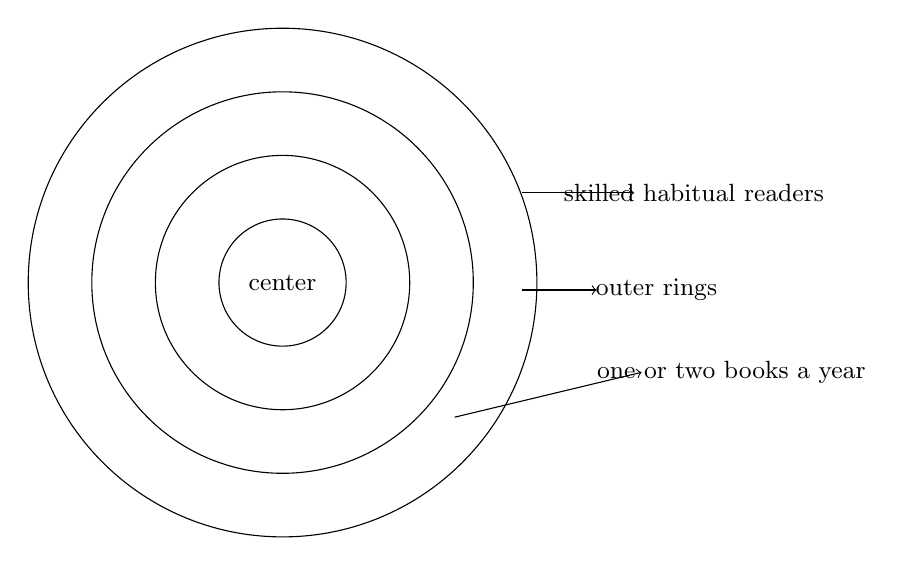
\begin{tikzpicture}[scale=0.95]
\draw (0,0) circle (0.85);
\draw (0,0) circle (1.7);
\draw (0,0) circle (2.55);
\draw (0,0) circle (3.4);
\node at (0,0) {\small center};
\node at (5.5,1.2) {\small skilled habitual readers};
\draw[->] (3.2,1.2) -- (4.7,1.2);
\node at (5.0,-0.1) {\small outer rings};
\draw[->] (3.2,-0.1) -- (4.2,-0.1);
\node at (6.0,-1.2) {\small one or two books a year};
\draw[->] (2.3,-1.8) -- (4.8,-1.2);
\end{tikzpicture}
\end{figure}

The design constraint is therefore
\begin{equation}
\text{style must satisfy center} \quad \& \quad \text{style must carry outskirts}.
\end{equation}

\subsection{Question \& Answer}

\paragraph{Question.} How do we write for both expert readers and people who barely read at all?

\paragraph{Answer.} Not by writing two books, but by making one style do double duty. At the center the style can be appreciated \emph{as} style. At the outskirts the style must be useful. It must guide, ease, and carry. Child's own image is physical: it is as if the writer had a hand gently on the reader's back, pushing that reader through the book without making the pressure felt as pressure.

This is the exact point at which the lecture introduces propulsion. A book is not one sentence but thousands in sequence. Hence the local law:
\begin{equation}
\text{sentence rhythm}_1 \to \text{sentence rhythm}_2 \to \cdots,
\qquad
\Delta p_{\text{sentence}} > 0 \text{ small but persistent}.
\end{equation}
Here \(p\) is merely an editorial name for forward pressure. The lecturer's point is simpler: each sentence must trip forward. The increase is subtle, almost hidden. Child compares it to a pop song whose tempo accelerates slightly as it goes, or to a polished carnival chute from which there is no elegant exit once one is inside.

This is why one of the compliments he values most is so concrete: ``I finished it.'' To the habitual reader this may sound modest. To the outer-ring reader it may register as real achievement. Propulsion, then, is not merely a stylistic virtue. It is the mechanics by which a book gets the reader all the way through.

\section{Question Engines, Cliffhangers, and Dialogue Illusion}

Once propulsion has been named, the host performs the lecture's next useful service. He refuses to let propulsion remain a single grand word. He presses it into smaller mechanisms. Does it live only in sentences? Does it also live in questions, in chapter endings, in the held-open gap between what is known and what is not yet known? Child answers by moving from prose back to television, and from television back to prose again.

\subsection{Question \& Answer}

\paragraph{Question.} How do questions and rhythm actually pull a reader through a book?

\paragraph{Answer.} By activating a lack. Once a real question has been planted, the audience wants the answer. That desire then carries attention across time, across breaks, and across chapters.

The basic chain is
\begin{equation}
\text{implied question} \Longrightarrow \text{answer withheld} \Longrightarrow \text{reader / viewer retention}.
\end{equation}

The host's question about cliffhangers then lets Child derive the mechanism historically:
\begin{equation}
\text{switching cost} \downarrow \Longrightarrow \text{need for sharper hooks} \uparrow.
\end{equation}

The worked derivation is one of the clearest in the lecture:
\begin{enumerate}
\item In the earlier television world, leaving a channel cost real effort.
\item That friction created inertia; the viewer might stay through a break simply because changing channels was inconvenient.
\item The remote control collapsed the switching cost.
\item Once the cost fell, inertia no longer protected attention.
\item Therefore producers had to place a live question before the break and delay the answer.
\item The same principle transfers into fiction: the chapter ending becomes not a pause alone, but a question under tension.
\end{enumerate}

Child dramatizes the point by performing it. He says that by 1990 viewers possessed something they had not possessed in 1980. The host, and we with him, now want the answer. Only once the appetite is active does the answer arrive: the remote control. This is why Child concludes, in this restricted and technical sense, that plotting difficulty is often overestimated. Once a genuine question has been posed, the reader will stay to learn the answer.

The lecture then widens the effect from mechanics to experience. A good book makes the reader angry to put it down and eager to return. Child offers a Christmas anecdote in which he half-wished the family schedule would be delayed so he could keep reading. The host gives the right word for the state: absorption. Child answers with his preferred word: immersion. The point is not merely speed. It is the making of a world hard to leave.

At this stage the host introduces a seemingly opposite principle: perhaps the way to achieve this is not to try too hard. Child agrees. He cites David Mamet's account of actors who do not step onstage asking to be liked, but arrive with a self-possession that says, in effect, take me or leave me. The same applies to writing. Likability, if designed too explicitly, becomes neediness.

The host then asks the question that the chapter must keep: how can such insouciance coexist with discipline? Child's answer is the lecture's most explicit paradox:
\begin{equation}
\text{writing as art} = 100\%, \qquad
\text{writing as job} = 100\%.
\end{equation}
He calls this mathematically impossible, and that is precisely the point. The writer must believe both propositions wholly: that the work belongs to an artistic tradition, and that the work is a job for which family, publisher, retailer, and reader all create obligations. That paradox is not an afterthought. It is the emotional and practical structure beneath the whole lecture.

When the conversation later restarts on a smaller scale, the host begins not with plot or audience but with the main character. The question is likability. Child's answer is perfectly continuous with the Mamet principle. A main character cannot be engineered to be hated, but cannot successfully be engineered to be liked either. What matters is authenticity. Reacher, as Child first conceived him, was in many respects a barbarian. The clue was simply that Child liked him. Since readers share more culture than they do not share, that private response was not a proof, but it was a plausible signal.

\subsection{Question \& Answer}

\paragraph{Question.} How do we make prose feel natural while actually engineering it for motion and emphasis?

\paragraph{Answer.} By remembering that literal transcription is not realism. Real speech is disordered. Written dialogue must therefore be artificial, but artificial in such a way that the reader experiences it as natural.

Child states the principle with great force:
\begin{equation}
\text{real speech} \neq \text{written dialogue},
\qquad
\text{written dialogue is structured artifice that must feel unstructured}.
\end{equation}

Real conversation is full of fragments, placeholders, false starts, and long dead spaces. Yet if we copied it faithfully, the page would not live. So the craft problem is not to record speech, but to construct the illusion of speech. Rhythm does part of the work. Stress does part of the work. Repetition does part of the work.

The host's train anecdote gives Child an explicit example:
\begin{equation}
\text{``I need my money''}, \qquad \text{``I lost my money''}
\Longrightarrow
\text{need / lost / money rise as stress points.}
\end{equation}

The derivation is simple and exact:
\begin{enumerate}
\item The repeated noun \emph{money} stays in the ear.
\item The emotional state strips away ornamental language.
\item The verbs \emph{need} and \emph{lost} now carry the change of pressure.
\item The resulting line sounds more spoken precisely because it has been more carefully controlled.
\end{enumerate}

Child adds a useful technical caution. One may use italics for emphasis in extremis, but a page peppered with italics soon becomes typographical noise. Better to construct the rhythm so that the line lands on the intended word by itself. The continuity with propulsion is now visible. At the chapter level, at the sentence level, and inside dialogue, the task is the same: engineer pressure without exposing the machinery.

\section{Beginnings, Endings, and the Monster Outline in the Head}

The lecture now broadens again, but in a revealing way. The host asks about beginnings and endings in the book. Child first answers at the scale of a life. Most aspiring writers, he says, are too early. Enthusiasm and talent may be present, but content is not yet there. One should read, live, accumulate. Only then does the smaller question return: where does the book itself begin, and where does it stop?

The rules are severe and memorable:
\begin{equation}
\text{do not start when the earth cooled} \Longrightarrow \textit{in medias res},
\end{equation}
\begin{equation}
\text{story over} \Longrightarrow \text{book over}.
\end{equation}

The first attacks the novice habit of burying the live present under explanatory backstory. We do not need everything first. We need something active now. The second attacks the equally novice impulse to keep wrapping after closure has already occurred. Child gives the striking example of believing he still had more to write, and then realizing suddenly that the book had already ended.

The lecture then revisits television from a different angle. Once television ceased to be a concentrated activity and became a parallel one, producers began compensating for distraction by redundancy. They would tell you that they were about to tell you, then tell you, then tell you that they had told you. Child recognized the temptation to carry too much of that habit into prose. He began instead to leave more inferential work to the reader. Information would be present, even plain, but the final assemblage would not always be performed on the page.

That turn matters because it prepares the lecture's next answer. If one leaves more work to the reader, one is relying on structure. But where is that structure if it is not in the outline?

\subsection{Question \& Answer}

\paragraph{Question.} If there is no written outline, where does structure come from?

\paragraph{Answer.} From the internalization of many thousands of prior structures. Child's point is not that he creates without form. It is that the form has already been absorbed. Reading has installed it.

We may write the claim as
\begin{equation}
\text{tens of thousands of books read} \Longrightarrow \text{internal database of plots, characters, cliffhangers, structures}.
\end{equation}

So the more careful reconstruction is
\begin{equation}
\text{improvisation} + \text{massive prior reading} \Longrightarrow \text{implicit structural control}.
\end{equation}

This is why the phrase ``monster outline'' is so useful. Child denies the paper outline, but affirms the internal one. The host helps here by supplying analogies from other arts, designers, musicians, filmmakers, all of them consuming far more than outsiders suppose. Child immediately confirms the diagnosis. Writers are not primarily writers. They are primarily readers.

His late ratio makes the point with almost comic clarity:
\begin{equation}
\text{books written per year} \ll \text{books read per year}.
\end{equation}

That is the answer to the no-outline puzzle. Structure is not absent. It is distributed through memory, habit, genre knowledge, and long exposure. The writer is drawing from an immense filing system even when the drawing feels spontaneous.

\section{Violence, Character Shorthand, and the Limits of Teaching}

The final movement gathers several topics that might at first look miscellaneous. They are not. Each returns to the same thesis: fiction works by stylized selection, not by literal copying.

Violence is the clearest late example. Child says that violence in narrative is, once again, an illusion. Real violence is usually brief, ungainly, and followed by significant after-effects. The screen version in which blows are exchanged back and forth with endless recoverability is almost never realistic. So why does the reader want it? The lecture answers by paradox.

\begin{equation}
\text{civilized commitment to due process} + \text{private retaliatory desire}
\Longrightarrow
\text{fictional violence as release}.
\end{equation}

Readers believe in law, safeguards, rights, and civilization. They do not want the real world reordered around vengeance. But they also know the private flash of retaliatory desire. Fiction offers a release under protected conditions. The reader knows the world is fictional, and therefore can enjoy the satisfaction without wanting to inhabit it socially. The violence section is partially garbled in the transcript, but its stable structure is clear enough: real violence is brief and costly; fictional violence is stylized because it is serving psychic release rather than documentary fidelity.

The same selective logic then appears in characterization. Clothing, shoes, hair, teeth: these become fast visual operators. A gray ponytail with double denim, or the opposite stiffness of lace-up shoes and pleated chinos, may place a person quickly. Teeth can do the same. Child remarks that he had been doing this instinctively before a dentist reader made him notice it. The technical point is not that character reduces to wardrobe or dentition. It is that fiction often needs efficient, high-yield signals.

\subsection{Question \& Answer}

\paragraph{Question.} Can writing actually be taught, or only learned through long exposure?

\paragraph{Answer.} Child draws a real distinction. Much around writing can certainly be taught: the business, the pitfalls, the professional handling. But the central art, in his view, is not straightforwardly teachable. It may nonetheless be learnable. One can read, listen, live, and slowly internalize what no short formula could successfully hand over.

This answer fits the entire lecture. Dialogue is learned by listening. Structure is learned by reading. Character is sharpened by watching. Even the final answers about national storytelling cultures return us to this point. Scotland, in Child's account, builds alternative culture against the concentration of power. Ireland provides something else: the gift of a chance. If one begins telling a story in the pub, the room will hear a few seconds before judging. That small allowance is culturally enormous. It trains the storyteller to seize the floor, justify it quickly, and keep it.

The lecture closes, then, not on a rule but on a condition of growth. One learns to write by entering a world dense with stories, forms, and listeners, and by becoming answerable to them.

\section{Summary}

The lecture's order is itself the lesson. We begin with scale, because scale immediately raises the problem of plausibility. From there we move to geography, from geography to place as temperature and key, and from place to the anti-outline claim. Improvisation then proves not to be emptiness, but a mode backed by reading. The lecture widens again into audience, transaction, and the rings of readership, and from that widened view derives propulsion, question-hooks, cliffhangers, and the pressure of the sentence. It then restarts locally at character and dialogue, before moving outward once more to beginnings, endings, violence, shorthand characterization, and the limits of teaching.

The strongest unifying claim is that writing is never one thing only. It is local and large-scale, spontaneous and disciplined, readerly and writerly, artistic and occupational. That is why the closing paradox is not decorative but exact. Child asks us to hold two apparently incompatible truths at once, and the whole lecture has been an extended demonstration of how that can be done.